\chapter[Teoretická část studentské práce]{Teoretická část studentské\\ práce}

\section{Principy pořizování rentgenových snímků}
Pořizování rentgenových snímků je prováděno pomocí zdroje rentgenového záření, rentgenovaného objektu a detektoru rentgenového záření. Rentgenové záření jsou elektromagnetické vlny s vlnovou délkou od \SI{10}{\nano\meter} do \SI{1}{\pico\meter} jejichž enerigie se nejčastěji pohybuje od \SI{1}{\kilo\eV} do \SI{200}{\kilo\eV}. Toto elektromagnetické záření vzniká buď při přechodu elektronů mezi vnitřními vrstvami těžších atomů -- charakteristické X-záření, nebo při dopadu a prudkém zabrzdění elektronů na anodu -- brzdné záření. \cite{AstroNuklFyzika-JadRadFyzika}

Jak již bylo zmíněno výše, scéna pro pořizování rentgenových snímků (\cref{fig:x-ray-scene}) se skládá ze zdroje rentgenového záření, rentgenovaného objektu a detektoru rentgenového záření. Zdroj rentgenového záření ozařuje elektromagnetickým vlněním o vlnové délce \SI{5}{\pico\meter} až \SI{50}{\pico\meter} rentgenovaný objekt. V závislosti na tloušťce a absorpčních vlastnostech objektu se část záření absorbuje a zbylá část záření dopadá na detektor rentgenového záření. Výstupem detektoru je poté obraz ve stupních šedi.

\begin{figure}[bh]
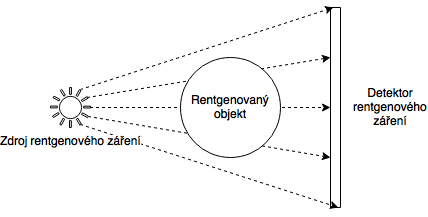
\includegraphics[width=\textwidth]{xray-scene}
\caption{Scéna pro pořizování rentgenových snímků.}
\label{fig:x-ray-scene}
\centering
\end{figure}